\documentclass[12pt,fleqn]{jreport}
\usepackage[dvipdfmx]{graphicx}
%\usepackage{epsbox}
\usepackage{graphics,latexsym}
\usepackage{ascmac}
\usepackage{amsfonts}
\usepackage{amsmath}
\usepackage{nccmath}
\usepackage{amsthm}
\usepackage{amssymb}
%\usepackage{epsbox}
\usepackage{float}
\usepackage{here}
\usepackage{lscape}
\usepackage{longtable}
\renewcommand{\bibname}{参考文献}
\usepackage{geometry}
\usepackage{subcaption}
\usepackage{multicol}

\topmargin         3mm  % トップとヘッダの間隔
\headheight        0mm  % ヘッダの高さ
\headsep           0mm  % ヘッダとテキストの間隔
\textwidth       170mm  % テキストの幅
\textheight      245mm  % テキストの高さ
\oddsidemargin  -2.5mm  % サイドとテキストの間隔(奇数ページ)
\evensidemargin -2.5mm  % サイドとテキストの間隔(偶数ページ)

\pagestyle{plain}

\begin{document}
\thispagestyle{empty}
\begin{center}
  {\Huge 卒 業 研 究 論 文}
\end{center}
\vspace{2cm}
\begin{center}
  {\huge 2022 年度}
\end{center}
\vspace{2cm}
\begin{flushleft}
  {\LARGE 題  目 }
\end{flushleft}
\begin{center}
  {\LARGE \underline{陸上競技の長距離種目における}\\
    \vspace{0.2cm}
    \underline{最適な練習組合せ}}\\
\end{center}
\vspace{0.5cm}
\begin{flushleft}
  {\LARGE 英文題目 }
\end{flushleft}
\begin{center}
  {\LARGE \underline{Optimal practice combinations }\\
    \vspace{0.2cm}
    \underline{for long distance events in track and field}
  }\\
\end{center}
\vspace{3cm}
\begin{flushleft}
  {\Large 指導教員 \underline{ 池辺 淑子准教授,西田 優樹助教 }}\\
  \vspace{5mm}
  {\Large 氏  名 \underline{ 照永 詩恩  }}\\
  \vspace{5mm}
  {\Large 学籍番号 \underline{ 4619060 }}
\end{flushleft}
\vspace{1.5cm}
\begin{flushright}
  {\Large 東京理科大学 工学部 情報工学科}\\
\end{flushright}
\newpage
\thispagestyle{empty}

\begin{center}
  {\huge 卒業論文要旨}
\end{center}
\vspace{3cm}
\large
今日,学生や一般市民が多くのスポーツ競技に参加しているが経験豊富な指導者の指導が受けられない人が存在する.
その場合は,本人自らが練習メニューを決めなければならない.試合で良い結果を出すためには,適切な量と質の練習を行う必要がある.
しかし,試合で良い結果を出すためのトレーニングメニューの調整をするのが容易ではない.
トレーニングに関する理論としてBanisterを中心とした研究グループによって提案された,
フィットネス,疲労,パフォーマンスを数理モデル化したフィットネス疲労理論というものが存在する.この理論
はトレーニングをすると身体にプラスなフィットネスと身体にマイナスな疲労の2要素が引き起こされ両者の和を
とるとパフォーマンスが算出されるという考え方に基づく理論である.
本研究では,陸上競技の長距離種目を例にとり,フィットネス疲労理論を用いて練習メニューの作成を数理計画問題として定式化した.
走力を向上させるために
パフォーマンスを低下させずにフィットネスを向上させるようなパラメータの設定をシミュレーション等を通して調べた.
その定式化されたものを解き出力された練習メニューを実施して実際に行われた試合にどのような影響が出たのかを検証したところ,
ピーキングはあっていたが走力を向上しなかったという結果が得られた.
%\cite{fitfig}
\newpage
\thispagestyle{empty}

\begin{center}
  {\huge Abstract}
\end{center}
\vspace{3cm}
Today, there are students and citizens who participate in sports but don't have access to experienced coaches.
In the case, they must decide their own training menu.
It is necessary to practice with appropriate amount and quality in order to achive good results in games.
However, it is not easy to adjust traning menus to achive good results in games.
As a theory of training, the "Fitness-Fatigue" existed from the 1970s to the 1990s, when a group of researchers led by Banister developed a mathematical model of fitness, fatigue, and performance.
This theory is based on the idea that training causes two factors: fitness, which is positive for the body, and fatigue, which is negative for the body, and that the sum of the two is used to calculate performance.
In this thesis, using the example of long-distance track and field events, this theory was formulated through simulation to create an optimal training menu with the goal of improving fitness without decreasing performance in order to improve running ability.
When the formulation was solved and the output practice menu was implemented to verify how it affected the actual game, the results showed that the peaking was correct but did not improve the running ability.


\newpage
\pagenumbering{roman}   %目次ページ番号のスタイル
\setlength{\baselineskip}{20pt}   %行間幅
\tableofcontents   %目次を付ける
\newpage
\listoffigures   %図目次を付ける
\listoftables   %表目次を付ける
\clearpage   %目次と本文を分ける
\pagenumbering{arabic}   %本文ページ番号のスタイル
%%%%%これ以下, 本文%%%%%
\newpage
\chapter{はじめに}
\large
今日,学生や一般市民が多くのスポーツ競技に参加している.
近年,運動やスポーツをする人が減っているとはいえ,令和3年度の「スポーツの実施状況等に関する世論調査」
によると20000件の標本のうち56.5\%が週1日以上運動やスポーツをしていて,半分以上の人が実施しているといえる\cite{sports1}.
運動やスポーツをする目的は様々である.例えば運動不足解消であったり体力増進・意地をしたいなどの理由がある.
その中でも自己記録や能力を向上させたいという人もいる.このような人たちは経験豊富な指導者を受けるべきである.
しかし,経験豊富な指導者の指導が受けられる人は少ない.令和3年度の中学校と高等学校における調査によると,
学校運動部部活動の指導者をしている人の中で経験がないが顧問をしている,経験はあるが実技指導力が不足しているという人が存在する\cite{sports2}.
経験豊富な指導者の指導が受けられない場合は,本人自らが練習メニューを決めなければならない
一方で試合で良い結果を出すためには,適切な量と質の練習を行う必要がある.一般的に強度が高い練習を継続していくほど
疲労は蓄積し,試合で満足のいく結果が出せなくなってしまう.逆に,強度の低い練習ばかり実施したり
全く練習をしなかったりすると競技力の不足によって同じく試合で満足のいく結果が出せなくなる.
このように試合で良い結果を出すためのトレーニングメニューの調整をするのが容易ではない.トレーニングに関する理論として1970年から1990年代にかけてBanisterを中心とした研究グループによって
フィットネス,疲労,パフォーマンスを数理モデル化したフィットネス疲労理論というものが存在する\cite{bani}.
フィットネス疲労理論は,トレーニングをすると
身体にプラスなフィットネスと身体にマイナスな疲労の2要素が引き起こされ両者の和を
とるとパフォーマンスが算出されるという考え方に基づく理論である.
本研究では,陸上競技の長距離種目を例にフィットネス疲労理論を用いて最適なトレーニングメニューの作成を定式化する.
\newpage
\chapter{問題設定}
本研究ではフィットネス疲労理論\cite{bani}を用いて
陸上競技長距離種目を例にパフォーマンスを低下させずにフィットネスを向上させて走力を向上させる目的とする.
\vspace{1cm}
\section{フィットネス,疲労,パフォーマンス}
\begin{figure}[h]
  \begin{center}
    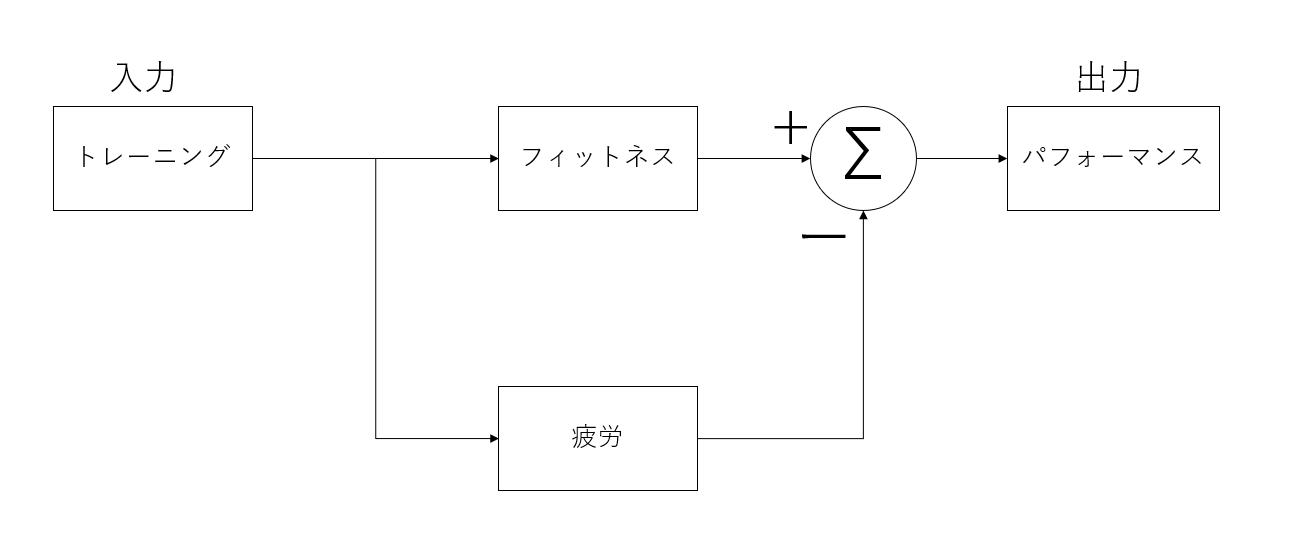
\includegraphics[width=15cm,height=5cm]{1.png}
  \end{center}
  \caption{フィットネス疲労理論の概念図}
\end{figure}
フィットネス疲労理論とは,時刻$t$において投与されたインプット$w(t)$のトレーニング負荷は,
正の効果をもたらすフィットネス$g(t)$と,負の効果をもたらす疲労$h(t)$が
拮抗して生体応答を引き起こし,両者の和としてパフォーメンス$p(t)$
がアウトプットされるというものである.この概要を図式化したものが図\ 2.1である.
時刻$t$におけるトレーニング負荷関数$w(t)$は競技によって異なるが,フィットネスと疲労
とパフォーマンスを表す関数$g(t),h(t),p(t)$は以下のとおりである.
\begin{eqnarray}
  g(t)&=&w(t)+g(t-i)e^{-\frac{1}{\tau_1}}\label{eq:fit1}\\%(2)
  h(t)&=&w(t)+h(t-i)e^{-\frac{1}{\tau_2}}\label{eq:fig1}\\%(3)
  p(t)&=&k_1g(t)-k_2h(t)\label{eq:per1}%(4)
\end{eqnarray}
ここで,Banister\cite{fitfig}が1991年に提唱したものに従い,パラメータを次のように設定する.
\begin{eqnarray}
  \tau_1&:&フィットネスの時定数であり\tau_1=45と設定\nonumber\\
  \tau_2&:&疲労の時定数であり\tau_2=15と設定\nonumber\\
  k_1&:&フィットネスの重みづけ係数でありK_1=1と設定\nonumber\\
  k_2&:&疲労の重みづけ係数でありk_2=2と設定\nonumber\\
  i&:&tまでのトレーニング期間であり本研究ではi=1と設定\nonumber
\end{eqnarray}

\section{トレーニング負荷}
また,トレーニング負荷$w(t)$の算出方法はいくつかある.例えば平均心拍数と最大心拍数を用いて求める方法や,
サッカーにおいてそれぞれのトレーニングメニューの内容によって定められている強度と実施時間で求める方法などがある\cite{fitfig1}.
本研究では対象とする陸上競技長距離種目とし以下のものとする.\\
\begin{eqnarray}
  w(t)&=&ランニング強度(au)\times 距離(km)\times 路面係数\times 天候係数\label{eq:w1}%(5)
\end{eqnarray}\\
それぞれの各係数については以下のとおりで文献\cite{fitfig1}のものを用いる.
\begin{description}
  \item[ランニング強度係数(表\ 2.1)]  \\
        1kmあたりのペースによって値が定まり,速ければ速いほど値は大きくなる
  \item[路面係数(表\ 2.2)]  \\
        走る路面によってそれぞれ値が定められている.走る路面の種類にはトラック,ロード,グラウンドがある
  \item[天候係数(表\ 2.3)]  \\
        晴か雨なのか,また暑いのか涼しいのかによって値が定まるものである
\end{description}
\vspace{1cm}
\begin{longtable}{|c|c|c|c|}
  \caption{1kmあたりのペースとランニング係数}       \\
  \hline
  ペース(1km)      & 強度 & ペース(1km)      & 強度 \\
  \hline
  $\sim$5'00"      & 1.0  & 3'05$\sim$3'01"  & 8.5  \\
  \hline
  4'59"$\sim$4'00" & 1.5  & 3'00"$\sim$2'56" & 10.0 \\
  \hline
  3'59"$\sim$3'41" & 3.0  & 2'55$\sim$2'51"  & 11.0 \\
  \hline
  3'40"$\sim$3'33" & 3.5  & 2'50"$\sim$2'46" & 12.0 \\
  \hline
  3'32"$\sim$3'29" & 4.0  & 2'45$\sim$2'41"  & 16.0 \\
  \hline
  3'28"$\sim$3'21" & 4.5  & 2'40$\sim$2'36"  & 20.0 \\
  \hline
  3'20"$\sim$3'11" & 5.0  & 2'35"$\sim$      & 24.0 \\
  \hline
  3'10"$\sim$3'06" & 8.0  &                  &      \\
  \hline
\end{longtable}
\begin{longtable}{|c|c|}
  \caption{路面係数}    \\
  \hline
  路面       & 路面係数 \\
  \hline
  トラック   & 1.00     \\
  \hline
  ロード     & 1.10     \\
  \hline
  グラウンド & 1.25     \\
  \hline
\end{longtable}
\newpage
\begin{longtable}{|c|c|}
  \caption{天候係数}      \\
  \hline
  天候         & 天候係数 \\
  \hline
  晴れ・暑い   & 1.30     \\
  \hline
  晴れ・涼しい & 1.00     \\
  \hline
  雨・暑い     & 1.35     \\
  \hline
  雨・涼しい   & 1.10     \\
  \hline
\end{longtable}
\newpage
\chapter{定式化}

陸上競技の長距離種目における,トレーニングメニュー作成問題定式化の最適化問題として定式化する.
\vspace{1cm}
\section{フィットネス,疲労,パフォーマンス}
トレーニングの$t$日目におけるフィットネス,疲労,パフォーマンスを表す関数$g(t)$,$h(t)$,$p(t)$を具体的に記述する.
まず,トレーニング開始時刻を1日目として$t$日目のフィットネスの関数$g(t)$を求めていく.
1日目から順に(\ref{eq:fit1})式についてを整理し展開していったもの以下の表に示す.
\begin{longtable}{|c|c|}
  \caption{各時刻におけるフィットネス関数}                                 \\
  \hline
  時刻     & フィットネス                                                  \\
  \hline
  1        & $w(1)$                                                        \\
  \hline
  2        & $w(2)+w(1)e^{-\frac{1}{45}}$                                  \\
  \hline
  3        & $w(3)+w(2)e^{-\frac{1}{45}}+w(1)e^{-\frac{2}{45}}$            \\
  \hline
  $\vdots$ & $\vdots$                                                      \\
  \hline
  $t$      & $w(t)+w(t-1)e^{-\frac{1}{45}}+\cdots+w(1)e^{-\frac{t-1}{45}}$ \\
  \hline
\end{longtable}
表\ 3.1より$t$日目におけるフィットネスの関数$g(t)$を整理すると,
\begin{eqnarray}
  g(t)&=&\sum_{i=1}^t w(i)e^{-\frac{t-i}{45}}\label{eq:fit2}%(6)
\end{eqnarray}
次に疲労であるがフィットネスと同じ方法で求められる.よって$t$日目における疲労の関数$h(t)$は以下のようになる.
\begin{eqnarray}
  h(t)&=&\sum_{i=1}^t w(i)e^{-\frac{t-i}{15}}\label{eq:fig2}%(7)
\end{eqnarray}
最後にパフォーマンスであるが(\ref{eq:per1})式に$k_1=1$,$k_2=2$を代入するだけである.よって時刻$t$におけるパフォーマンスの関数$p(t)$は以下のようになる.
\begin{eqnarray}
  p(t)&=&g(t)-2h(t)\label{eq:per2}%(4)
\end{eqnarray}
\section{記号の定義 }
定式化においては$i$日目の第$j$メニューについて,
\begin{eqnarray}
  A_{ij}&:&i日目における第jメニューのランニング強度\nonumber\\
  R_{ij}&:&i日目における第jメニューの路面係数\nonumber\\
  W_{ij}&:&i日目における第jメニューの天候係数\nonumber
\end{eqnarray}
を定数にする.
そして変数を,
\begin{eqnarray}
  x_{ij}&:&i日目における第jメニューを実施するか否か(バイナリ変数)\nonumber\\
  D_{ij}&:&i日目のおける第jメニューの距離(整数値)\nonumber
\end{eqnarray}
と設定する.
\vspace{1cm}
\section{陸上競技の長距離種目における最適なトレーニングメニューを求める定式化}
トレーニング期間を全体で$T$日とし,あらかじめ定める$k$種類のメニューの中から各日1つを選択するものとする.
設定した定数,変数を用いて定式化すると次のようになる.
\vspace{1cm}
\begin{eqnarray}
  \mathop{\rm maximize}&\ \ &\sum_{i=1}^T (\sum_{j=1}^k A_{ij}D_{ij}R_{ij}W_{ij}x_{ij})e^{-\frac{T-i}{45}}\label{eq:max}\\%(10)
  \mathop{\rm subject\ to}&\ \ &\sum_{j=1}^k x_{ij}\leq 1\ \ (i=1,\cdots , T)\label{eq:st1}\\%(11)
  &&p(i)\geq P\ \ (i=i_1,\cdots , i_s)\label{eq:st3}%(13)
\end{eqnarray}
\vspace{1cm}
ここで,(\ref{eq:max})式は目的関数でありフィットネスを最大化する.
(\ref{eq:st1})式は各トレーニング日に高々1つのメニューに実施することを示している.
(\ref{eq:st3})式は特定の$i_k$日目にパフォーマンスがあらかじめ定める$P$より下がらないことそ示している.
\newpage
\chapter {数値実験}
\vspace{1cm}
2022年12月5日に開催された試合に向けた11月21日から12月4日のトレーニンングメニューの作成を定式化し,
実際にPythonとGurobiを用いて解き,出力された解を実施して12月5日の試合にどのような影響を
及ぼしたのかを検証する.
\section{予備実験}
この実験ではトレーニングメニューの確定とパフォーマンスの下限を確定させた.
\subsection{メニューの確定}
メニューの確定についてはPythonを用いてシミュレーションを行った.
シミュレーションは日数を31とし4つのパターンを行った.
\begin{enumerate}
  \item ジョグのみ
  \item ペース走を導入
  \item インターバル走を導入
  \item 休みを導入
\end{enumerate}
細かなメニューについては過去に実施したメニューの中から適当に選んだ.
それぞれのシミュレーションを実行した結果は以下の通りになった.
\begin{table}[H]
  \caption{シミュレーションの結果}
  \begin{center}
    \begin{tabular}{|c|c|c|c|}
      \hline
        & 最終日のフィットネス & 最終日の疲労 & 最終日のパフォーマンス \\
      \hline
      1 & 373.40               & -431.92      & -58.82                 \\
      \hline
      2 & 500.84               & -611.18      & -110.34                \\
      \hline
      3 & 521.18               & -613.47      & -92.29                 \\
      \hline
      4 & 384.55               & -459.22      & -74.67                 \\
      \hline
    \end{tabular}
  \end{center}
\end{table}
\begin{figure}[H]
  \begin{tabular}{cc}
    \begin{minipage}[t]{0.45\hsize}
      \centering
      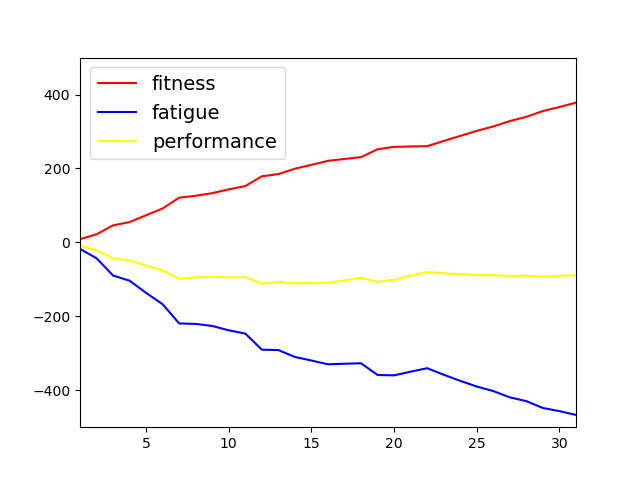
\includegraphics[scale=0.5]{sim1.png}
      \caption{シミュレーション1}
    \end{minipage} &
    \begin{minipage}[t]{0.45\hsize}
      \centering
      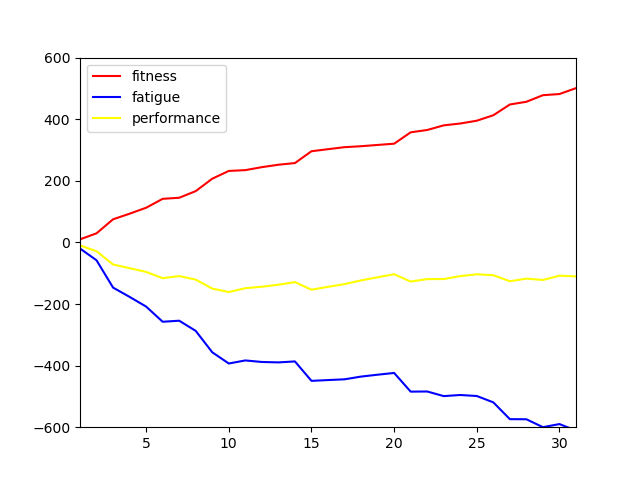
\includegraphics[scale=0.5]{sim2.png}
      \caption{シミュレーション2}
    \end{minipage}   \\
    \begin{minipage}[t]{0.45\hsize}
      \centering
      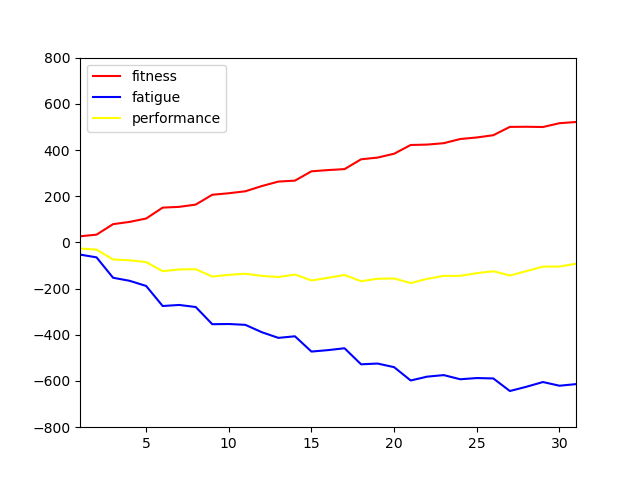
\includegraphics[scale=0.5]{sim3.png}
      \caption{シミュレーション3}
    \end{minipage} &
    \begin{minipage}[t]{0.45\hsize}
      \centering
      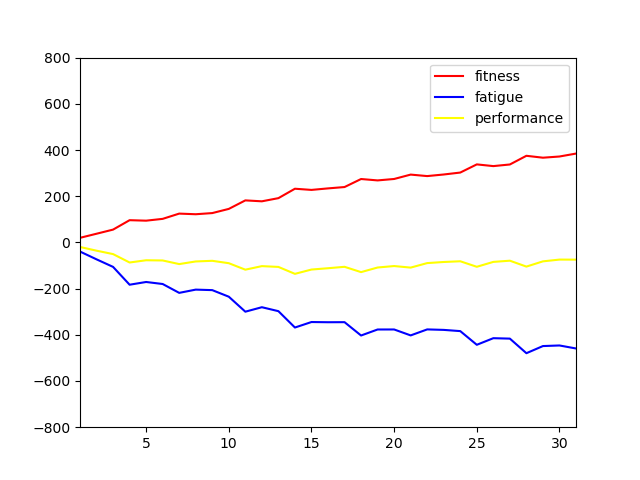
\includegraphics[scale=0.5]{sim4.png}
      \caption{シミュレーション4}
    \end{minipage}   \\
  \end{tabular}
\end{figure}
\newpage
結果からフィットネスを向上させるにはジョグに加えてペース走やインターバルといったポイント練習も加えることが大事だとわかった.
しかし,その一方で疲労がたまりパフォーマンスが非常に低下している.トレーニングを実施しない日を作ることで
疲労やパフォーマンスはトレーニングを毎日実施しているものと比べて疲労は溜まらずパフォーマンスも低下していない.
したがって,メニューについてはジョグとペース走とインターバルをすべて用いかつ休みも導入するということにした.
細かなメニューについては,当時の体の状態を見てその時期付近で走り切れているメニューに絞った.
\subsection{パフォーマンスの下限}
(\ref{eq:st3})式の$P$の値を決定する.試合で良い結果を出すためにはポイント練習が大事になる.
なので,直近でポイント練習を走り切れたときと走り切れなかったときでその14日前のシミュレーションを行ってみた.出力された結果は以下のとおりである.
\begin{table}[H]
  \caption{ポイント練習2週間前のパフォーマンス}
  \begin{center}
    \begin{tabular}{|c|c|c|}
      \hline
        & ポイント練習ができたか(Yes or No) & 前日のパフォーマンスの値 \\
      \hline
      1 & Yes                               & -97.11                   \\
      \hline
      2 & No                                & -101.06                  \\
      \hline
      3 & No                                & -104.20                  \\
      \hline
    \end{tabular}
  \end{center}
\end{table}
表\ 4.2よりポイント練習を走り切れるときと走り切れないときの違いはポイント練習前日のパフォーマンスが約$-100$を下回らないことが分かった.
\section{設定}
\vspace{1cm}
トレーニングメニューについては,自身が実施したことのあるトレーニングメニューをまず準備し,
シミュレーション等を通して検討した結果,4つに絞った.メニューの詳細は表\ 4.3のとおりである.
\newpage
\begin{longtable}{|c|c|c|c|}
  \caption{実施するトレーニングメニュー}                                   \\
  \hline
  メニュー                         & トレーニング強度$(A)$ & 路面係数$(R)$ \\
  \hline
  速いジョグ                       & 1.0                   & 1.1           \\
  \hline
  遅いジョグ                       & 1.5                   & 1.1           \\
  \hline
  10000mペース走(ポイント練習)     & 3.5                   & 1.0           \\
  \hline
  $1000$m$ \times 5$(ポイント練習) & 8.0                   & 1.0           \\
  \hline
\end{longtable}
天候係数については季節は冬なので全て1とする.またトレーニングメニューにおける
ポイント練習は走力の向上に直結する高強度の練習であり,ジョグはジョギングの略称であり
長距離の基礎の部分を作るトレーニングである.表\ 4.3,(\ref{eq:w1})式を基に$w(t)$は以下のように定めた.
\begin{eqnarray}
  w(i)&=&(1.1x_{i1}+16.5x_{i2})D_{i}+35x_{i3}+40x_{i4}\label{eq:w3}
\end{eqnarray}
各項ランニング強度,距離,路面係数,天候係数とそのメニューを実施するか否かの変数の積になるが,
10000mペース走,$1000$m$\times 5$の距離は$D_{i3}=10$,$D_{i4}=5$で固定し,速いジョグ$D_{i1}$と遅いジョグの距離$D_{i2}$の距離は1種類のメニューのみとしたため
$D_{i1}=D_{i2}=D_i$と設定した.また,それぞれのポイント練習実施の回数,日付をあらかじめ指定した.
具体的には10000mペース走を11月23日,11月27日に,1000m$\times$5は11月30日に行うことにしたので,
$x_{3,3}=x_{7,3}=x_{10,4}=1$とした.
\section{定式化}
4.1節および4.2説をふまえ,定式化(\ref{eq:max})式$\sim$ (\ref{eq:st3})式を以下のように変更した.
\newpage
\begin{eqnarray}
  \mathop{\rm maximize}&\ \ &\sum_{i=1}^{13} \left((1.1x_{i1}+16.5x_{i2})D_{i}+35x_{i3}+40x_{i4}\right)e^{-\frac{13-i}{45}}\label{eq:max1}\\%(10)
  \mathop{\rm subject\ to}&\ \ &\sum_{j=1}^4 x_{ij}\leq 1\ \ (i=1,\cdots,13)\label{eq:st12}\\%(11)
  &&8\leq D_{i} \leq 12\ \ (i=1,\cdots,13) \label{eq:st2}\\%(12)
  &&p(i)\geq -100\ \ (i=7,9,13)\label{eq:st32}\\%(13)
  &&\sum_{i=1}^{13} x_{i1}+x_{i2}\geq 5\label{eq:st42}\\%(14)
  &&\sum_{i=1}^{13} x_{i1}\geq 1\label{eq:st52}\\%(15)
  &&\sum_{i=1}^{13} x_{i4}=2\label{eq:st6}\\%(16)
  &&\sum_{i=1}^{13} x_{i7}=1\label{eq:st7}\\%(17)
  &&x_{i4}=1\ \ (i=3,7)\label{eq:st8}\\%(18)
  &&x_{i5}=1\ \ (i=10)\label{eq:st9}%(19)
\end{eqnarray}
\newpage
各式の説明は次のとおりである.
\begin{itemize}
  \item (\ref{eq:st32})式は(\ref{eq:st3})式をポイント練習の前日,もしくは当日に$-100$を下回らないように設定した.
  \item (\ref{eq:st2})式はジョグの距離の範囲を8km$\sim$12kmに定めた.
  \item (\ref{eq:st42})式はジョグの実施回数を5回以上に定めた.
  \item (\ref{eq:st52})式は速いジョグの実施回数を1回以上に定めた.
  \item (\ref{eq:st6})式,(\ref{eq:st7})式はそれぞれのポイント練習の回数の設定であり10000mペース走は2回,1000m$\times$5は1回と定めた.
  \item (\ref{eq:st8})式,(\ref{eq:st9})式はポイント練習の時刻設定であり上記設定のように定めた.
\end{itemize}
\vspace{1cm}
(\ref{eq:st3})式の定数$P$は,シミュレーションより$-100$と定めている.時刻については前日か当日に設定した.
\section{実行環境及び計算計測時間}
\vspace{1cm}
計算環境とプログラム計算計測時間を以下に示す.
\begin{center}
  \begin{multicols}{2}
    \begin{description}
      \item[OS$\cdots$Windows\ 11]
      \item[CPU$\cdots$Intel\ Core\ i7\ (1.8GHz)]
      \item[メモリ$\cdots$8.0GB]
      \item[言語$\cdots$python\ 3.8.5]
      \item[ソルバー$\cdots$Gurobi\ 9.5.2]
      \item[ 実行時間(5回の平均)$\cdots$0.354s]
    \end{description}
  \end{multicols}
\end{center}
\newpage
\section{結果}
\vspace{1cm}
\begin{longtable}{|c|c|c|c|}
  \caption{出力されたメニュー}                                   \\
  \hline
  日付     & メニュー       & 日付     & メニュー                \\
  \hline
  11月21日 & 12km速いジョグ & 11月28日 & 9km速いジョグ           \\
  \hline
  11月22日 & 12km速いジョグ & 11月29日 & 8km(9km)遅いジョグ      \\
  \hline
  11月23日 & 10000mペース走 & 11月30日 & 1000m$\times$5\         \\
  \hline
  11月24日 & 12km速いジョグ & 12月1日  & 10km遅い(9km速い)ジョグ \\
  \hline
  11月25日 & 11km遅いジョグ & 12月2日  & 10km(9km)遅いジョグ     \\
  \hline
  11月26日 & 休養           & 12月3日  & 休養                    \\
  \hline
  11月27日 & 10000mペース走 & 12月4日  & 試合                    \\
  \hline
\end{longtable}
実施した試合の結果と自己ベストについては以下の表のとおりである.
\begin{table}[H]
  \caption{試合の結果と自己ベスト}
  \begin{center}
    \begin{tabular}{|c|c|c|}
      \hline
                            & 試合の結果 & 自己ベスト \\
      \hline
      距離                  & 8.4km      & 5km        \\
      \hline
      タイム                & 28分7秒    & 16分00秒   \\
      \hline
      1kmの平均ラップタイム & 3分20秒    & 3分12秒    \\
      \hline
    \end{tabular}
  \end{center}
\end{table}
実施したメニューは定式化のミスがあり最終的に出力されたメニューとは若干違うものになってしまった.
表\ 4.4のカッコ内のものが実施したメニューとなる.試合に出場した結果,現在の自分の持っている力をすべて出し切ることができたと考えられる.
したがって,ピーキングはあっていたとみなすことができる.一方では表\ 4.6より自己ベストの平均ラップタイムより8秒遅く距離は長いが目標にしていた
ペースは3分15秒だったので走力が向上しているとは言えなかった.
\newpage
\chapter{考察}
\vspace{1cm}
試合で現在の自分の持っている力をすべて出し切ることができたことから,出力された結果はピーキングには非常に適したものだということが考えられる.
定式化するうえでいろいろと試してみたところ,ジョギングの距離やポイント練習の内容,日付,その期間に実施する回数を指定しなければ2日間や3日間で
ポイント練習が一塊となってバランスの悪いメニュー構成になったりジョグの距離が今のレベルでは走ることができないような距離が出力されたりと
納得のいくトレーニングメニュー構成を出力することができなかった.そのため定式化においては,経験に基づくある程度の事前の決定は必要である.
試合ではピーキングはあっていたものの走力が向上しているとはいえなかったので短期間では走力は向上するものではないため定式化する際のトレーニング期間を
$T=30$などといった長い期間での実施をするべきであり,それに応じて自分のレベルをシミュレーションや過去のトレーニングデータを基にして知り,制約条件を
設定していくべきだと考えた.
\newpage
\chapter{まとめと今後の課題}
\vspace{1cm}
本研究では,フィットネス疲労理論を用いてパフォーマンスを低下させすぎずにフィットネスを向上させていくことを目標にしてきた.
ポイント練習が散らばっており,ジョグの距離が走り切ることが可能なトレーニングメニュー構成となる解を得るためには自分のレベルをシミュレーション
を通して知り,トレーニングメニューの種類を絞り,日付や距離の範囲を絞るったうえで定式化することが大事である.また,実験結果より最終的な出力結果
とは若干違うメニュー構成のトレーニング実施になってしまったがピーキングにはあったいた.その一方で,走力が向上するというようなメニュー構成ではなかった.
\par 今後の課題としては走力を向上させるために定式化を変更させる必要がある.期間の増加,ジョグの距離の増加が考えられる変更点である.また,それに応じて
納得のいくメニュー構成が立てられるようにシミュレーションや過去のデータの分析を通して制約式を考えていくことが大切になる.

\newpage
\begin{flushleft}
  {\Huge\textbf{謝辞}}
\end{flushleft}
\vspace{2cm}
本研究を進めるにあたり、多大なご指導、ご助言をいただいた池辺淑子准教授、西田優樹助教には大変お世話になりました。心より感謝と御礼申し上げます。
\newpage
\begin{thebibliography}{99}
  \bibitem{bani}Morton R.H.,Fitz-Clarke J.R. , and Banister E.W. (1990) Modeling human performance in running. J Appl Physiol. 69(3)pp.: 1171-1177.
  \bibitem{fitfig}Banister E.W. (1991) Modeling elite athletic performance. In: Green H.J., McDugal J.D., and Wenger H. (ed). Physiological testing of elite athletes. Human Kinetics, Campaign IL. pp 403-424.
  \bibitem{fitfig1}「フィットネスー疲労モデル」を用いたトレーニング刺激と生体応答のモニタリングとパフォーマンス予測,URL(https://system5-site-one.ssl-link.jp/sandcplanning/uploads/solution/20/5b14a2d1f169020.pdf),閲覧日2023年1月20日
  \bibitem{sports1}「令和3年度スポーツの実施状況等に関する世論調査」結果の概要,URL(https://www.mext.go.jp/sports/content/20220222-spt\_kensport01-000020451\_1.pdf),閲覧日2023年1月20日
  \bibitem{sports2}学校運動部活動指導者の実態に関する調査報告書,url(https://www.japan-sports.or.jp/Portals/0/data/katsudousuishin/doc/R3\_houkokusho.pdf),閲覧日2023年1月20日
\end{thebibliography}
\end{document}